\chapter{Efficiencies}
\label{sec:Efficiencies}

The detection and reconstruction of particle decys is not perfect at all, i.e. not all particles and tracks happening in succession of a \proton\proton interaction are detected and recorded.
This discrepancy between the measured signal yields and the actually happened decays is summarized with the term ``efficiencies".
There are several reasons why different kinds of efficiencies occur.
Here are some examples:
\begin{itemize}
    \item Particles are flying out of the detector.
    \item A particle traverses a sensor in the deadtime, i.e. a signal caused by an earlier particle is still processed. 
          In this time, the sensor isn't able to process the second signal.
    \item Applying cuts for the reduction of background prevents signal events to pass these cuts as well
    \item ...
\end{itemize}
It's obvious that this list above is only the tip of the iceberg.
Nonetheless it's crucial to account for these efficiencies if one measures a physical quantity reliant on the number of events.
The way how the efficiencies for the \LbToDpmunuX and \LbToLcmunu enter the measurement of the relative branching ratio \R is shown in equation (\ref{eq:R}).

The determination of the efficiencies requires the use of simulations.
These simulation samples contain informations about all generated events as well as reconstructed events after the simulation of the detector. 
The naive way would be to divide the number of reconstructed MC events after applying all selection cuts and divide this by the number of generated events. 
This efficiency is hereafter called selection efficiency \effSel.
Nonetheless, the generation of the events isn't efficient at all. 
Several requirements are already applied during generation to reduce the computation time of the simulation production.
Above all the simulation of the detector takes a lot of time.
That's why all generated events are required to be in the \lhcb aceptance.
A further acceleration of the production process can be achieved with additional requirements on the final state particles' (transverse) momenta.
Concerning the \LbToDpmunuX and \LbToLcmunu channel these requirements are different and likewise the efficiencies of the generation process.
Thus, the so called generator level efficiency \effGen also has to determined for both channels. 
The total efficiency used for the calculation of \R is then the product $\effGen \cdot \effSel$.

As life is not that easy the simulations don't perfectly describe the data. 
Above all the \LbToDpmunuX signal simulation doesn't contain a proper physics description and is thus in disagreement with data. 
Unfortunately, no theory prediction of the \LbToDpmunuX channel is available to fix this problem.
The plots in figure \ref{fig:reweighting} show a comparison of data (black points) and the simulation (red lines).
To get a better description of the decay the simulation hence has to be reweighted.
This should lead to a more proper estimate of the efficiency.
Several reweigthing steps are applied and will be described in the following.
\begin{figure}[hptb]
	\centering
	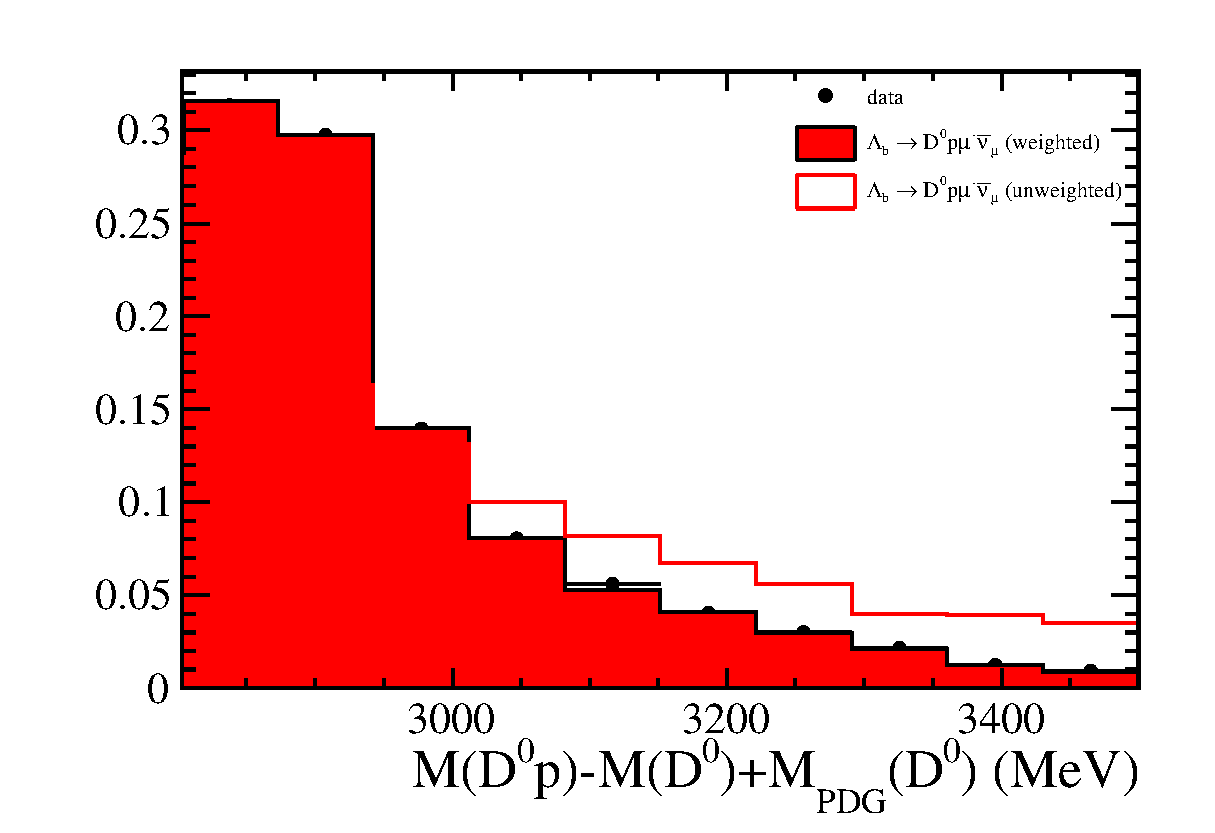
\includegraphics[width=0.49\textwidth]{LbToD0p/comparisons/3D/mD0p_mD0mu_mD0pmu/20Bins/20.0MaxWeight/Bh_DELTA_MASS}
	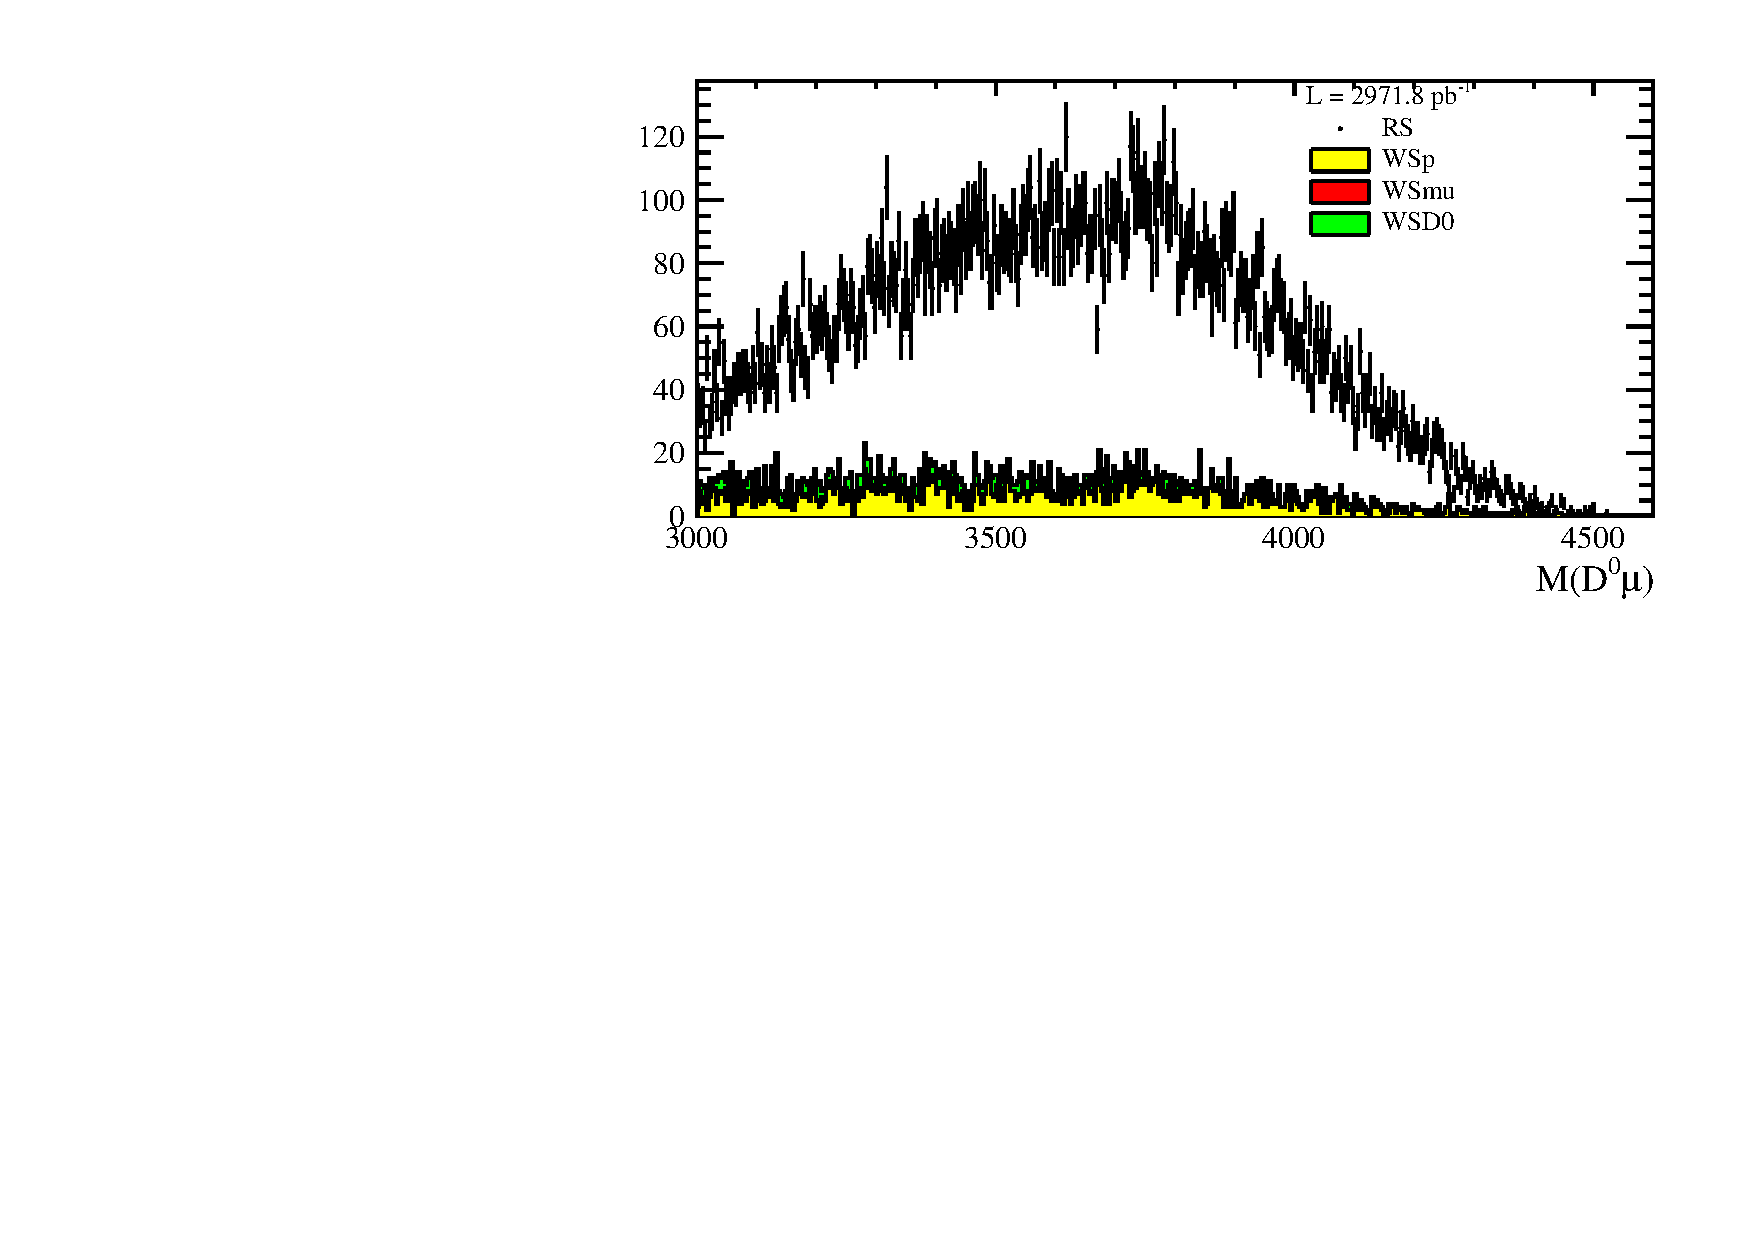
\includegraphics[width=0.49\textwidth]{LbToD0p/comparisons/3D/mD0p_mD0mu_mD0pmu/20Bins/20.0MaxWeight/B_M}
	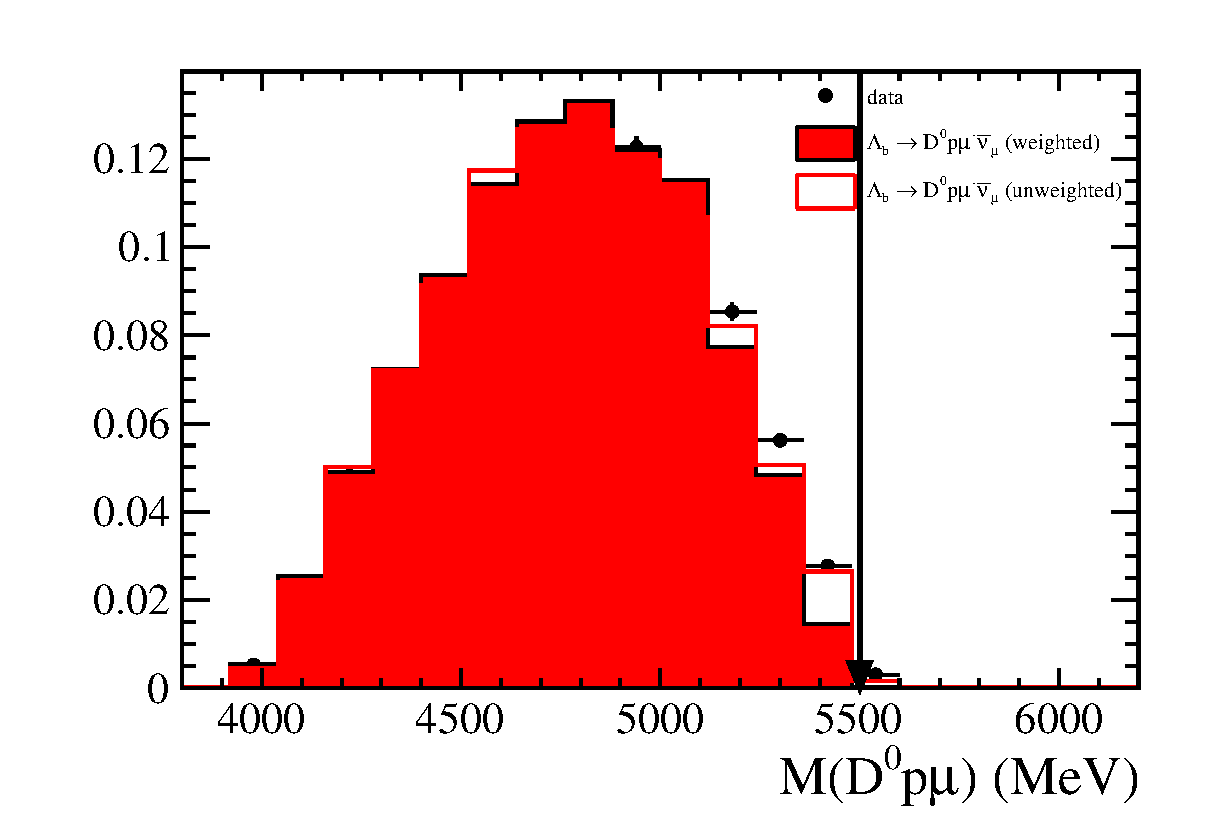
\includegraphics[width=0.49\textwidth]{LbToD0p/comparisons/3D/mD0p_mD0mu_mD0pmu/20Bins/20.0MaxWeight/Bh_M}
	\caption{Comparison of data (black points) and simulation for the \LbToDpmunuX channel before (red line) and after (red shaded area) threedimensional reweighting as described in the text (see sec. \ref{sec:Reweight_D0p}).}
	\label{fig:reweighting}
\end{figure}

\section{Kinematic reweighting of the \LbToDpmunuX and \LbToLcmunu channel}
The production of \Lb baryons depends strongly on their transverse momentum as figure \ref{fig:LbPTrew} (left) from ref. \cite{Lb_production_kinematic} shows. 
This dependence isn't well emulated in the simulation and has thus to be corrected. 
This was already done in the semileptonic \lhcb-measurement of $|\Vub|$ in ref. \cite{SL_Vub} using the decay \decay{\Lb}{\jpsi\Dz\proton}. 
To calculate the weights they compared data and simulation of this hadronic \Lb decay channel, shown in figure \ref{fig:LbPTrew} (right). 
In this analysis, the used weights are determined from the same channel with the help figure \ref{fig:LbPTrew} (right).
The reweighting is applied in both, \LbToDpmunuX and \LbToLcmunu, channels according to the true \Lb transverse momentum \pt, i.e. the actual generated transverse momentum.
\begin{figure}[hptb]
	\centering
	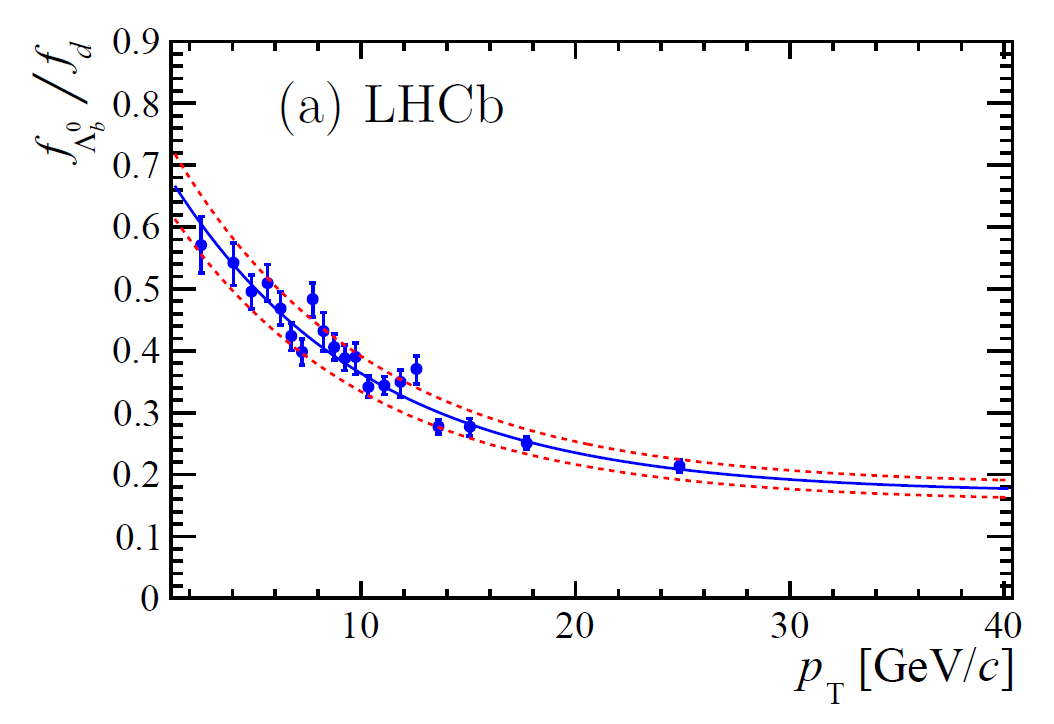
\includegraphics[width=0.49\textwidth]{Lb_production_pt_dependence}
	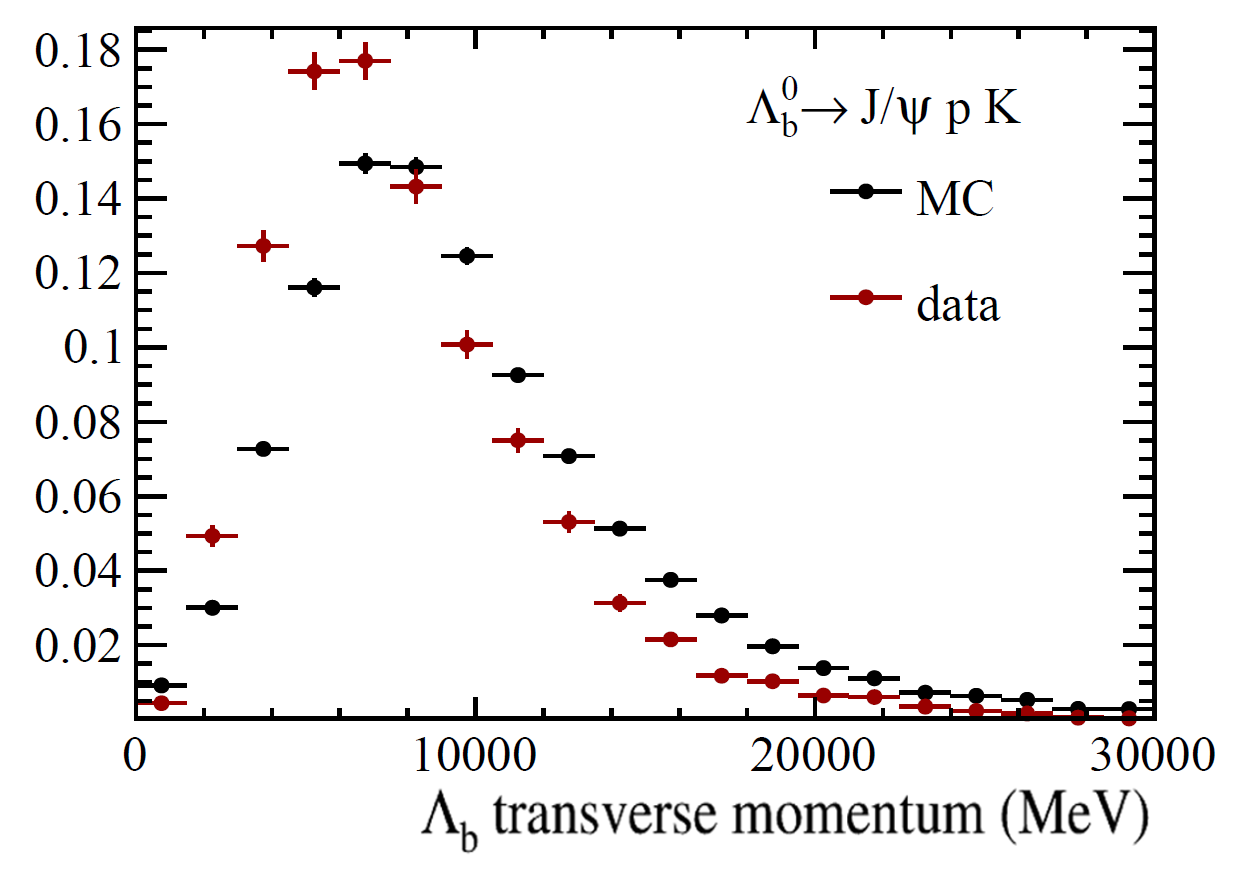
\includegraphics[width=0.49\textwidth]{Lb_pt_comparison_weights}
	\caption{Left: Ratio of \Lb to \Bd production as a function of \pt. Figure taken from \cite{Lb_production_kinematic}.  Right: Transverse \Lb momentum for \decay{\Lb}{\jpsi\Dz\proton} decays in data and simulation. Figure taken from the documentation belonging to \cite{SL_Vub}.}
	\label{fig:LbPTrew}
\end{figure}


\section{Reweighting of the \LbToDpmunuX decay simulation}
\label{sec:Reweight_D0p}
It has already been mentioned that the underlying physics in the \LbToDpmunuX simulation is wrong.
Since there aren't any theoretical predictions on that channel, the reweighting of the simulation has to be done carefully.
To come as close to data as possible, a threedimensional reweighting in the variables
\begin{itemize}
    \item M(\Dz\proton)
    \item M(\Dz\mun)
    \item M(\Dz\proton\mun)
\end{itemize}
has been chosen. 
This choice is not trivial and above all obvious, but there are several reasons for it:
\begin{enumerate}
    \item The simulation is completely off from the data distribution in these variables.
    \item These variables are already available at generator level, i.e. before the detector response is simulated. 
          To calculate the selection efficiency the simulation has to be reweighted at generator stage as well.
    \item There aren't any selection requirements on these variables. 
          Otherwise, no weights could be assigned to ones not fulfilling the requirements at generator level
          \footnote{There exists a selection requirement on M(\Dz\proton\mun) in this analysis to eliminate \decay{\Lb}{\Dz\proton\pim} background, but less than 0.5\% of all events have their generated mass above this value. 
                    Thus, its impact on the efficiency can be neglected.}.
\end{enumerate}
After the description of the reweighting and efficiency calculation process, it should become clear why these three points are important:
\begin{itemize}
    \item \textbf{Determination of the weights} \\
          There are two normalized threedimensional histograms drawn for both, generated events (in the following called MCDecayTreeTuple or MCDTT) and events after reconstruction, applying selection cuts and the kinematic reweighting (DecayTreeTuple or DTT). 
          Both histograms have the three variables mentioned above on their axes.
          The histogram with the weights is now calculated by dividing the DTT histogram through the MCDTT histogram.
    \item \textbf{Assigning weights to the events} \\
          Now, this weight histogram is used to assign a weight to each DTT (\weight{DTT}) and MCDTT (\weight{MCDTT}) event.
          To get the correct bin in the weight histogram the generated masses \Mtrue{\Dz\proton}, \Mtrue{\Dz\mun} and \Mtrue{\Dz\proton\mun} are used.
    \item \textbf{Calculation of the efficiency} \\
          The efficiency can now be calculated with
          \begin{align}
              \epsilon = \frac{\sum \weight{DTT}}{\sum \weight{MCDTT}}, \label{eq:effrew}.
          \end{align}
          To account for the loss of statistical power due to reweighting, both numerator and denominator in equation (\ref{eq:effrew}) are multiplied by the renormalisation factor $\sum \weight{MCDTT} / \sum \weight{DTT}^2$. 
          This doesn't affect the central value of $\epsilon$ but influences the statistical error, which is calculated using binomial statistics.
\end{itemize}
It should now be clear, that with this procedure one must not cut on the weighting variables, since otherwise the weights outside the cut region would be zero. 
Hence it wouldn't be clear which weights have to be assigned to the MCDTT events. 
The distribution of the masses after reweighting are also shown in figure \ref{fig:reweighting}.
A decided improvement of the data description can be figured out.
Many more comparisons between data and simulation before and after reweighting can be found in the appendix \ref{app:Reweight_D0p} in figure \ref{fig:reweight_D0p_app}.
Having these reweighting steps in mind, it is now possible to calculate the efficiencies at different stages.

Concerning the channel \LbToLcmunu no further reweighting is applied since the agreement in the comparison between data and simulation seems to be sufficient.
Several comparison plots on this channel can be found in figure \ref{fig:reweight_Lc_app} in \ref{app:Reweight_Lc}.


\section{Generator level efficiencies}
As a reminder, generator level efficiencies arise due to the fact, that one demands the generated events to be in the \lhcb acceptance and apply some (loose) requirements on the kinematics to accelerate the simulation process.
The generator level samples are reweighted as described above: the \LbToLcmunu sample with the kinematic \pt(\Lb) reweighting and the \LbToDpmunu sample with both reweightings.
For signal and normalization channel the following generator level efficiencies are obtained:
\begin{align*}
    \effGenLc &= \effGenLcval \pm \effGenLcerr, \\
    \effGenDp &= \effGenDpval \pm \effGenDperr.
\end{align*}

\section{Reconstruction and selection efficiencies}
The reconstruction and selection efficiencies are calculated analogously.
The same reweighting procedure on the different samples is performed.
The results for signal and normalization channel are:
\begin{align*}
    \effSelLc &= \num[scientific-notation=true]{\effSelLcval \pm \effSelLcerr}, \\
    \effSelDp &= \num[scientific-notation=true]{\effSelDpval \pm \effSelDperr}.
\end{align*}

\section{Total efficiencies}
To summarise the values above the total efficiencies for the channels are:
\begin{align*}
    \effDp &= \effGenDp \cdot \effSelDp = \num[scientific-notation=true]{\effDpval \pm \effDperr}, \\
    \effLc &= \effGenLc \cdot \effSelLc = \num[scientific-notation=true]{\effLcval \pm \effLcerr}.
\end{align*}
For the consideration of systematics later it is sometimes more useful to consider the ratio of both efficiencies
\begin{align*}
    \frac{\effLc}{\effDp} = \effRatioval \pm \effRatioerr.
\end{align*}
